% Author: Alfredo Sánchez Alberca (email:asalber@ceu.es)
% Plot with the phases of the statistical cycle
\begin{tikzpicture}
\node[align=center, inner sep=10pt] (population) at (1,1) {\includegraphics[scale=0.5]{img/introduction/population}\\
Population}; 
\pause
\node[align=center, inner sep=10pt] (sample) at
(1,6){\includegraphics[scale=0.5]{img/introduction/sample}\\ Sample}; 
\draw[-stealth, redceu, line width=12pt] (population) -- (sample) node[midway,rotate=90,white]
{Sampling\quad\phantom{0}};
\pause
\node[align=center,  inner sep=10pt] (statistics) at (8,6) {\Large $\bar x$ \quad $s^2$\\\Large \quad $p$ \quad
$g_1$\\[5pt] summary\\ measures}; 
\draw[-stealth, redceu, line width=12pt] let \p1=(sample.east), \p2=(1,0) in (\x1+\x2,\y1) -- (statistics)
node[midway,white] {Descriptive\quad\phantom{0}}; 
\pause
\node[align=center, inner sep=10pt] (model) at (8,1) {\includegraphics[scale=0.5]{img/introduction/model}\\ Model };
\draw[-stealth, redceu, line width=12pt] (statistics) -- (model) node[midway,rotate=-90,white]
{Inferential\quad\phantom{0}};
\pause
\draw[-stealth, redceu, line width=12pt] (model) -- (population) node[midway,white] {\quad Prediction};
\end{tikzpicture}